\section{Introduction} \label{ch1}

\subsection{Course structure}

The exam is composed of the following parts:

\begin{itemize}
    \item a \textbf{written exam}, providing the \textbf{60\%} of the overall grade;
    \item the \textbf{discussion of a project} (software and report) or the \textbf{presentation of a paper}, providing the remaining \textbf{40\%} of the grade. For the discussion of a project, there may be 1 or 2 extra points for good projects.
\end{itemize}

\subsection{What Information Retrieval Is}
\textbf{Information retrieval (IR)} is about finding material (usually documents) of an unstructured nature (usually text) that satisfies an information need from within large collections (usually stored on computers). Information retrieval is fast becoming the dominant form of information access, overtaking traditional database-style searching. The first example of information retrieval system can be considered the \textit{Memex Machine} conceived by Vannevar Bush in the 30s, which actually cannot be classified as a real IR system, since it was more similar to a browsing hypertext system. In this sense, the principal driver of innovation for IR has been the World Wide Web, and in turn the continuous optimization of IR effectiveness, i.e. the quality of its results, and efficiency, i.e. the speed of the search, has driven web search engines to new quality levels.

Nowadays, the largest fraction of the data volume and the market cap is represented by \textbf{unstructured data}, i.e. data which has not a clear easy-for-a-computer structure, for example text documents etc.. An important factor for the growth of the volume of unstructured data has been the Web growth, along with the Web pages size growth and the search engine usage. In general, a \textit{Search Engine Result Page (SERP)} is not represented exclusively by an algorithmic search results, but also with images, videos, query suggestions and advertisements. More specifically, the agents involved in the Web search field are the \textit{users}, who try to access the information and request relevance and speed, the \textit{search engine}, which tries to attract more users, to increase the ads revenues and to reduce the operational costs, and the advertisers, which wants to attract the users to their sites by paying little money. In general, the Web Search Engine is composed of three major components, as represented in Picture \ref{web_search}:

\begin{itemize}
    \item the \textit{web crawling} phase;
    \item the \textit{indexing} phase;
    \item the \textit{query processing} phase.
\end{itemize}

\begin{figure}[h!]
		\centering
		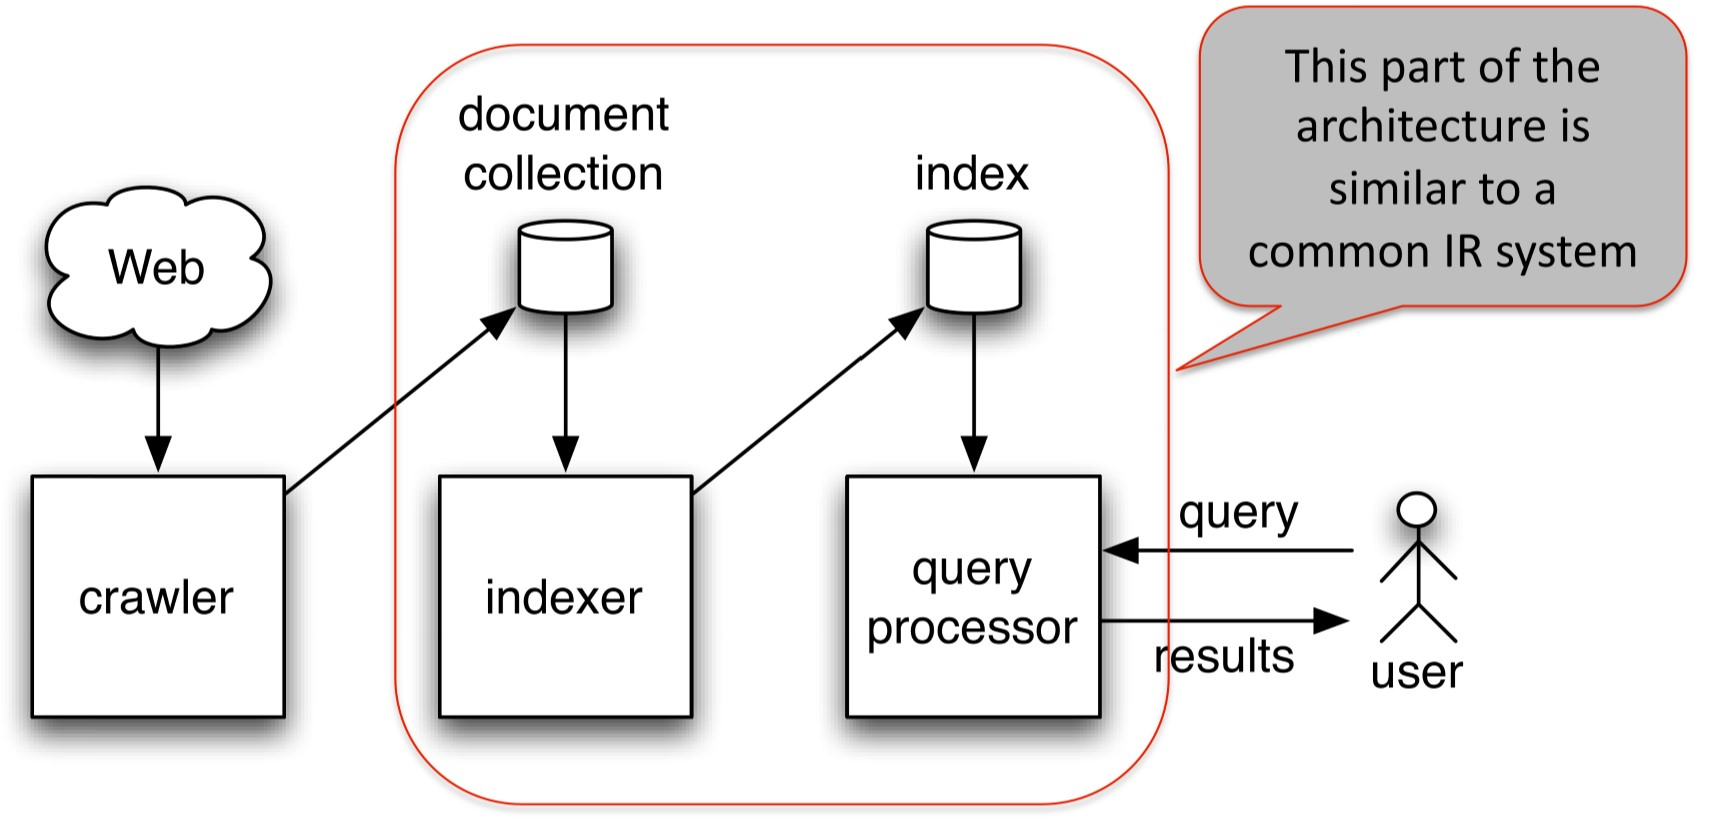
\includegraphics[scale = 0.6]{img/web search engine.jpg}
		\label{web_search}
\end{figure}

\subsection{Basic assumptions}
A \textbf{collection} is a set of documents, that we assume to be static at the moment, and the goal of IR is to retrieve documents with information that is relevant to the user's information need and helps the user to complete a task. In order to evaluate the quality of the retrieved documents, we introduce two basic metrics:

\begin{itemize}
    \item the \textit{precision}, which represents the fraction of retrieved documents that are relevant the the user's information need;
    \item the \textit{recall}, which represents the fraction of all relevant documents in the collection that are retrieved.
\end{itemize}

